\documentclass[12pt,a4paper]{book} % article, report, book.
%%%%%%%%%%%%%%%%%%%%%%%%%%%%%%%%%%%%%%%%%%%%%%%%%%%%%%%%%%%%%%%%%%%
%%% Documento LaTeX                                             %%%
%%%%%%%%%%%%%%%%%%%%%%%%%%%%%%%%%%%%%%%%%%%%%%%%%%%%%%%%%%%%%%%%%%%
% Título: Paquetes
% Autor:  Ignacio Moreno Doblas
% Fecha:  2014-02-01
%%%%%%%%%%%%%%%%%%%%%%%%%%%%%%%%%%%%%%%%%%%%%%%%%%%%%%%%%%%%%%%%%%%
% Tabla de materias:
% 1 Codificación e idioma %
% 2 Matemáticas y Física %
% 3 Gráficos%
% 4 Estilo y formato%
%%%%%%%%%%%%%%%%%%%%%%%%%%%%%%%%%%%%%%%%%%%%%%%%%%%%%%%%%%%%%%%%%%%

%1 Codificación e idioma%
\usepackage[utf8]{inputenc} %Codificación en utf8%
\usepackage[spanish]{babel} %Hyphenation (Guionado) en español%
\usepackage[T1]{fontenc} %Codificación de fuente%
\usepackage{eurofont} %Tipografía euro (€)%

%2 Matemáticas y Física %
% Importante para ecuaciones, magnitudes y unidades%
\usepackage{amssymb,amsmath,latexsym,amsfonts} % paquetes estándar%
\usepackage[squaren]{SIunits} %Paquete para magnitudes y unidades físicas%
\usepackage{ifthen} %sentencias if y while%

%3 Gráficos%
\usepackage{graphics,graphicx} %paquetes gráficos estándar%
\usepackage{wrapfig} %paquete para gráfica lateral%
\usepackage[rflt]{floatflt} %figuras flotantes%
  % \begin{floatingfigure}[r]/[l]{4.5cm}
  % \end{floatingfigure}
\usepackage{graphpap} %comando \graphpaper en el entorno picture%

%4 Estilo y formato%
\usepackage{fancyhdr} %cabeceras y pies mejor que con \pagestyle{}%
\usepackage{titlesec,titletoc} %Formateo de secciones y títulos%
\raggedbottom %Para fragmentar versos en varias páginas%
\usepackage{makeidx} %MakeIndex%
%\usepackage{showidx} % Hace que cada comando \index se imprima en la página donde se ha puesto (útil para corregir los índices)
\usepackage{alltt} % Define el environment alltt, como verbatim, excepto que \, { y } tienen su significado normal. Se describe en el fichero alltt.dtx.
\usepackage[pdftex,bookmarksnumbered,hidelinks]{hyperref} %hyper-references%
\usepackage{minitoc} % Para poner tablas de contenido en cada capítulo.
\usepackage{listings} % Para escribir piezas de código C, Python, etc. %
%listings configuration
\lstset{
  language=[ARM]Assembler, %Puede ser C, C++, Java, etc.
  showstringspaces=false,
  formfeed=\newpage,
  tabsize=4,
  commentstyle=\itshape,
  basicstyle=\ttfamily,
  morekeywords={models, lambda, forms}
}

\usepackage{tipa} % tipografía IPA (International Phonetic Alphabet)
\usepackage{longtable} %Entorno Longtable, fracciona tablas a lo largo de páginas%
\usepackage{colortbl}
\usepackage{acronym}  %Para expandir automáticamente los acrónimos

%%%%%%%%%%%%%%%%%%%%%%%%%%%%%%%%%%%%%%%%%%%%%%%%%%%%%%%%%%%%%%%%%%%
% Tabla de materias:
% 1 Información del Documento %
% 2 Comandos a nivel de texto %
% 3 Comandos a nivel de entorno %
% 4 Comandos a nivel de página y sección %
% 5 Otros comandos %
%%%%%%%%%%%%%%%%%%%%%%%%%%%%%%%%%%%%%%%%%%%%%%%%%%%%%%%%%%%%%%%%%%%

% 1 Información del Documento %
\newcommand{\pfctitlename}{Guiones de prácticas sobre la plataforma Raspberry Pi}
\newcommand{\pfcauthorname}{Antonio José Villena Godoy}
\newcommand{\pfctutorname}{Rafael Asenjo Plaza \\ Francisco Javier Corbera Peña}
\newcommand{\pfcanno}{2015}

% 2 Comandos a nivel de texto %
\newcommand{\R}{\textsuperscript{\textregistered}}  %Símbolo registrado%
\newcommand{\C}{\textsuperscript{\copyright}} %Símbolo Copyright%
\newcommand{\TM}{\texttrademark} %Símbolo Trade Mark (marca comercial)%

% 2.1 Comandos abreviatura %
\newcommand{\tit}{\textit} %Fuente cursiva (itálica)%
\newcommand{\tbf}{\textbf} %Fuente negrita%
\newcommand{\ttw}[1]{\texttt{#1}} %Fuente máquina de escribir (typewriter)%
%Combinación%
\newcommand{\textittt}[1]{\textit{\texttt{#1}}} %itálica y typewriter%
\newcommand{\textittw}{\textittt} % Otra forma de escribirlo.
\newcommand{\tittw}{\textittw} %Shortened%
\newcommand{\tbftw}[1]{\tbf{\ttw{#1}}}

%Crea una nueva línea y la indenta sin crear interlineado extra.
\newcommand{\nli}{\\ \indent} 

%Para escribir un correo electrónico%
\newcommand{\mailto}[1]{\href{mailto:#1}{#1}}

% Si vas a hacer un uso básico de \index (entradas en el índice de sólo un nivel, sin formatos especiales, etc.), define la orden
\newcommand{\miindex}[1]{#1\index{#1}}

\newcommand{\hs}{\hspace} % Abreviatura espacio horizontal
\newcommand{\vs}{\vspace} % Abreviatura espacio vertical

% Abreviaturas para los conjuntos de números más comunes.
\newcommand{\realnumbers}{\mathbb R}
\newcommand{\naturalnumbers}{\mathbb N}
\newcommand{\integernumbers}{\mathbb Z}
\newcommand{\rationalnumbers}{\mathbb Q}
\newcommand{\complexnumbers}{\mathbb R}
\newcommand{\irrationalnumbers}{\mathbb I}

% Doble barra sobre una letra (para expresar las matrices).
\newcommand{\doublebar}[1]{\bar{\bar{#1}}} 
% Ej: \vector(y) = \doublebar(A) \vector(x) (Stma. lineal de ec.)

% 3 Comandos a nivel de entorno %
\newcommand{\benu}{\begin{enu}} % Begin enumerate
\newcommand{\eenu}{\end{enu}}   % End enumeration

%Comando para escribir código Python
\newcommand{\code}[3]{
  %\hrulefill
  %\subsection*{#1}
  %\subsubsection{#1}
  \lstinputlisting{#2}
  %#1\\
  \begin{table}[h!]
    \centering
    \caption{#1}
    \label{#3}
  \end{table}
  \vspace{2em}
}

% 4 Comandos a nivel de página y sección %
%Crea página en blanco
\newcommand{\blankpage}{\clearpage{\pagestyle{empty}\cleardoublepage}}

% Versión x del comando section: sin numeración pero sí aparece en la tabla de contenidos.
\newcommand{\sectionx}[1]{
  \section*{#1}
  \addcontentsline{toc}{section}{#1}
}

% Versión y del comando section: sin numeración y NO aparece en la tabla de contenidos.
\newcommand{\sectiony}[1]{
  \section*{#1}
}

% Versión x del comando chapter: sin numeración pero sí  aparece en la tabla de contenidos.
\newcommand{\chapterx}[1]{
  \chapter*{#1}
  %\addcontentsline{toc}{chapter}{#1} %Caused by minitoc package%
  \addstarredchapter{#1} %For minitoc package%
}

% substituto del comando \chapter: incluye estilo de página.
\newcommand{\chapterbegin}[1]%
  {%
    \pagestyle{fancy}
    \fancyhead[LE,RO]{\thepage}
    \fancyhead[LO]{Capítulo \thechapter. #1}
    %\fancyhead[RE]{Parte \thepart \rightmark} %
    \fancyhead[RE]{\nouppercase{\rightmark}} %
        
    \chapter{#1}
  }

% Versión x del comando \chapterbegin: sin numeración y aparece en la tabla de contenidos.
\newcommand{\chapterbeginx}[1]%
  {%
    \pagestyle{fancy}
    \fancyhead[RO,LE]{\thepage}
    \fancyhead[RE,LO]{#1}
    %\fancyhead[LO]{Chapter \thechapter}
    %\fancyhead[RE]{Part \thepart} %
    
    \chapterx{#1}
  }

%Fin de capítulo
\newcommand{\chapterend}{\pagestyle{empty}\cleardoublepage \thispagestyle{empty}}
%Si fuera un artículo en lugar un libro, \clearpage en lugar de \cleardoublepage

% 5 Otros comandos %
%\let\Oldpart\part
%\newcommand{\parttitle}{}
%\renewcommand{part}[1]{\Oldpart{#1}\renewcommand{\parttitle}{#1}} %Header customization%

%Cambiar el título índice de capítulo a ``Contenido''.
\renewcommand{\mtctitle}{Contenido}

\dominitoc % Para tablas de contenidos por capítulo.

\addto{\captionsspanish}{
  \renewcommand{\listtablename}{Índice de Tablas}
  \renewcommand{\tablename}{Tabla} } % Por ejemplo, modificar el nombre de 'Cuadro' a 'Tabla'.

\addto{\captionsspanish}{
  \renewcommand{\contentsname}{Índice} }

%Si se desea cambiar el tipo de letra a Arial
% por cualquier razón, descomentar las siguientes
% dos líneas
%\renewcommand{\rmdefault}{phv} % Arial
%\renewcommand{\sfdefault}{phv} % Arial
  
%\addto{\captionsspanish}{
% \renewcommand{\partname}{Fase} }

%\addto{\captionsspanish}{%
%    \renewcommand{\refname}{\vspace{-4.5ex}}} % Para que no aparezca el texto 'referencias' en la bibliografía.

% Modifica el interlineado
%\renewcommand{\baselinestretch}{1.5}

   \definecolor{myfboxbg}{gray}{0.9}
   \newsavebox{\efcaja}
   \newenvironment{myfbox}{\begin{lrbox}{\efcaja}}
               {\end{lrbox}{\colorbox{myfboxbg}{\usebox{\efcaja}}}}

%%%%%%%%%%%%%%%%%%%%%%%%%%%%%%%%%%%%%%%%%%%%%%%%%%%%%%%%%%%%%%%%%%%
% Tabla de materias:
%--------------------%
% 1 dobleindent
% 2 izqindent
% 3 dobleindentx
% 4 ite
% 5 descript
% 6 enu
% 7 itemization
% 8 sinopsis
% 9 objetivo
%%%%%%%%%%%%%%%%%%%%%%%
% Para conocer los parámetros de diseño de las listas, tales como
%  los márgenes izquierdo, derechos y los diferentes saltos,
%  véase el archivo ``List layout.png'' que acompaña esta plantilla.
% Así se conocerá mejor cómo adaptar un entorno según los requisitos 
%  del usuario.

%%%%%%%%%%%%%%%%%%%%%%%
% Definición de longitudes para usar en los entornos:
%
% Normal parskip.
\newlength{\parskipenv}
\setlength{\parskipenv}{\parskip}

\newlength{\parindentenv}
\setlength{\parindentenv}{\parindent}
%%%%%%%%%%%%%%%%%%%%%%%

% 1 dobleindent
%El entorno dobleindent está pensando para escribir párrafos con doble indentación a cada lado.
%Tiene dos parámetros de entrada con las distancias medidas desde los márgenes de página.

\newenvironment{dobleindent}[2]
  %Comienzo de nuevo entorno%
  {
  \begin{list}
    {}
    {
    % Left and right margins:
    \leftmargin = #1 
    \rightmargin = #2
    %
    % Separation from preceding and following text:
    \topsep = 0ex
    \partopsep = 0ex
    \parsep = \parskipenv
    %
    % Indentation for paragraphs:
    \itemsep = \parskipenv
    \itemindent = \parindentenv
    \listparindent = \itemindent
    %
    % Horizontal separation from label:
    \labelsep = 1ex
    \settowidth{\labelwidth}{0cm}
    }
    
     \item}
  % End new env
  {\end{list}}

%%%%%%%%%%%%%%%%%%%%%%%%%%%%%
%2 izqindent
% El entorno izqindent sólo crea un párrafo indentado a la izquierda.
\newenvironment{izqindent}[1]
{
\begin{dobleindent}{#1}{0cm}
}
{
\end{dobleindent}
}

%%%%%%%%%%%%%%%%%%%%%%%%%%%%%
% 3 dobleindentx
% El entorno dobleindentx es una variación del dobleindent usando leftskip y rightskip.
% Aunque es más limitado, también se puede usar.
\newenvironment{dobleindentx}[2] % Sólo funciona en modo paragraph
{ % Preamble
  \leftskip = #1
  \rightskip = #2
}
{ % Postamble
\leftskip = 0cm
\rightskip = 0cm
}

%%%%%%%%%%%%%%%%%%%%%%%%%%%%%
% 4 ite
% El entorno ite es una modificación del entorno itemize estándar de \LaTeX. Puede usarse o modificarse si el usuario lo desea.
% También puede parametrizarse el entorno enumerate o description de forma equivalente.
\newenvironment{ite}
  {
    \begin{izqindent}{\parindent}
    \hspace{-\parindent}  % compensación del sangrado que introduce el entorno.
    \vspace{-1.0\parskip} % compensación del \parskip que introduce el entorno.
    \vspace{-\baselineskip} % compensación por la línea que introduce el entorno.
    \begin{itemize}
  }
  {
    \end{itemize}
    \end{izqindent}
  }

%%%%%%%%%%%%%%%%%%%%%5
% commando stdformat para formatear los entornos descript, enu y itemization.
\newcommand{\stdformat}
  {% Declarations for format presentation.
    %     
    % Separation from preceding and following text:
    \setlength{\topsep}{0ex}%
    \setlength{\partopsep}{0ex} %
    %
    % Horizontal separation from label:
    \labelsep = 1ex
    \setlength{\labelwidth}{0ex}
    %
    % Left and right margins: 
    \setlength{\leftmargin}{1cm}%
    \addtolength{\leftmargin}{\labelsep}
    \setlength{\rightmargin}{0ex}
    %  
    % Indentation for paragraphs:
    \setlength{\itemindent}{-\leftmargin}%
    \addtolength{\itemindent}{1ex}
    \setlength{\listparindent}{\parindent}%
    %   
    % Separation between paragraphs.
    \setlength{\parsep}{\parskipenv}% 
    \setlength{\itemsep}{1ex}
  }

%%%%%%%%%%%%%%%%%%%%%%%%%%%%%
% 5 descript

\newenvironment{descript}
  % Beginning new env def.
  {
    \begin{list}
      {} % No default label for \item.
      {
        % Declarations for format presentation.
        \stdformat
        %
        \renewcommand{\makelabel}[1]{\normalfont\bfseries##1\hfil}
      }
  }
  % Ending new env def.
  {
    \hspace*{\fill} \\ \end{list}
  } % Se introduce un salto de línea para que el texto siguiente esté separado.
%END newenvironment{descript}

%%%%%%%%%%%%%%%%%%%%%%%%%%%%%
% 6 enu
\newcounter{itemnumber} % Counter for the environment.

\newenvironment{enu}
  % Beginning new env def.
  {
    \begin{list}
    {
      \raggedleft \arabic{itemnumber}
    }
    {
      \usecounter{itemnumber}
      \stdformat
    }
  }
  {
    \end{list}
  }

%%%%%%%%%%%%%%%%%%%%%%%%%%%%%
% 7 itemization
\newenvironment{itemization}
  % Beginning new env def.
  {
    \begin{list}
      {$\bullet$} % No default label for \item.
      {
        % Declarations for format presentation.
        \stdformat
      }
  }
  % Ending new env def.
  {
    \end{list}
  }


%%%%%%%%%%%%%%%%%%%%%%%%%%%%%
% 8 sinopsis
\newenvironment{sinopsis}{%[1]{
  \sectiony{Sinopsis}
  %\label{#1}
} {
  \pagebreak
}

%%%%%%%%%%%%%%%%%%%%%%%%%%%%%
% 9 objetivo
\newenvironment{objetivo}{%[1]{
  \sectiony{Objetivo}
  %\label{#1}
} {
}

%%%%%%%%%%%%%%%%%%%%%%%%%%%%%%%%%%%%%%%%%%%%%%%%%%%%%%%%%%%%%%%%%%%
% Tabla de materias:
%--------------------%
% 1 Márgenes de página
%%%%%%%%%%%%%%%%%%%%%%%
% Para conocer los parámetros de diseño de páginas, tales como
%  los márgenes izquierdo, derecho, anchura de página, etc.
%  véase el archivo ``Page layout.png'' que acompaña esta plantilla.
% Así se conocerá mejor cómo adaptar el documento según los 
%  requisitos del usuario.

% 1 Márgenes de página
%-------------------------------%
% Parámetros de estilo de página.
% DIN A4: 29.7 cm x 21 cm
%   área neta: 3 cm + 3 cm + 15 cm.
%
% Definición de márgenes de página
%  even para páginas pares
%  odd  para páginas impares
\newlength{\realoddsidemargin}    % \oddsidemargin menos 1 in.
\newlength{\realevensidemargin}   % \evensidemargin menos 1 in.
\newlength{\realtopmargin}        % \topmargin menos 1 in.
%
% Asignación de márgenes de página
% ASIGNESE en caso de querer cambiarlo
\setlength{\realtopmargin}{2cm}     % REAL top margin.
\setlength{\realoddsidemargin}{3cm}   % REAL oddside margin.
\setlength{\realevensidemargin}{3cm}  % REAL evenside margin.
\setlength{\hoffset}{0cm}
\setlength{\voffset}{0cm}
%
% Substracción de 1 pulgada de compensación
%  (véase ``Page Layout.png'' para más información)
\addtolength{\realoddsidemargin}{-1in}  % 1 inch = 2.54 cm.
\addtolength{\realevensidemargin}{-1in}
\addtolength{\realtopmargin}{-1in}
%
% Asignación de anchuras y márgenes
% No hay notas al margen
\setlength{\marginparsep}{0cm} % No van a existir notas al margen
\setlength{\marginparwidth}{0cm} % No van a existir notas al margen
%
% Asignación de anchura de texto
\setlength{\textwidth}{15cm}  % Anchura neta del texto (globalmente).
%
% Asignación de márgenes par, impar y en altura
\setlength{\oddsidemargin}{\realoddsidemargin}  % odd-page left margin (global).
\setlength{\evensidemargin}{\realoddsidemargin} % even-page left margin (global).
\setlength{\topmargin}{\realtopmargin}          % top margin (Global).

% Se puede usar también el paquete chngpage.

%%%%%%%%%%%%%%%%%%%%%%%%%%%%%%%%%%%%%%%%%%%%%%%%%%%%%%%%%%%%%%%%%%
%   1 Length commands.          %
%-------------------------------%
% Defines new length command (e.g., \newlength{\gnat}}
% \newlength{}
%
% Set lenght to a value.
% \setlength{\gnat}{length}
% \addtolength{}{}
%
% Sets the value of a length command equal to the width of a specified piece of text; e.g., \settowidth{\parindent}{\em small}.
% \settowidth{}{}
% Set the value of a height. e.g., \settoheight{\parskip}{Gnu}
% \settoheight{}{}
% Set the value that extends below the line. e.g., \settodepth{\parskip}{gnu}.
% \settodepth{}{}
%
% To multiply a length, write: 7.0\gnat = \gnat * 7.0
%%%%%%%%%%%%%%%%%%%%%%%%%%%%%%%%%%%%%%%%%%%%%%%%%%%%%%%%%%%%%%%%%%

\begin{document}

%%%%%%%%%%%%%%%%%%%%%%%%%%%%%%%%%%%%%%%%%%%%%%%%%%%%%%%%%%%%%%

\chapterbegin{Introducción al ensamblador}
\label{chp:IntrEnsam}
\minitoc

{\bf Objetivo}:
En esta sesión vamos a conocer el entorno de trabajo.
Veremos qué aspecto tiene un programa en ensamblador, veremos cómo
funcionan los tres programas que vamos a utilizar: el ensamblador,
el {\it enlazador (linker)} y el {\it depurador (debugger)}.
Del {\it debugger} sólo mostraremos unos pocos comandos,
que ampliaremos en las próximas sesiones.
También veremos la representación de los números naturales y de los
enteros, y el funcionamiento de algunas de las instrucciones del ARM.
Se repasarán también los conceptos de registros, flags e instrucciones
para la manipulación de bits.

\section{Lectura previa}

\subsection{Características generales de la arquitectura ARM}

ARM es una arquitectura RISC (Reduced Instruction Set Computer=Ordenador
con Conjunto Reducido de Instrucciones) de 32 bits, salvo la versión del
core ARMv8-A que es mixta 32/64 bits (bus de 32 bits con registros de 64
bits). Se trata de una arquitectura licenciable, quiere decir que la
empresa desarrolladora ARM Holdings diseña la arquitectura, pero son
otras compañías las que fabrican y venden los chips, llevándose ARM
Holdings un pequeño porcentaje por la licencia.

%\begin{figure}[h]
%  \centering
%    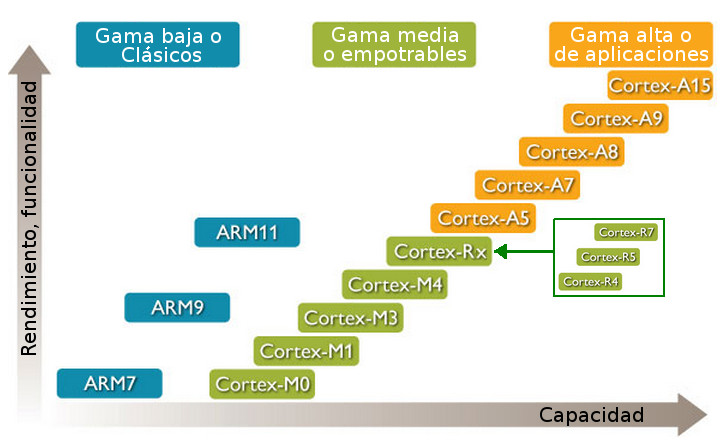
\includegraphics[width=13cm]{graphs/ArmRoadMap.jpg}
%  \caption{Clasificación de Familias ARM}
%  \label{fig:clasif_fami}
%\end{figure}

El chip en concreto que lleva la Raspberry Pi es el BCM2835, se trata de
un SoC (System on a Chip=Sistema en un sólo chip) que contiene además de
la CPU otros elementos como un núcleo GPU (hardware acelerado OpenGL
ES/OpenVG/Open EGL/OpenMAX y decodificación H.264 por hardware) y un
núcleo DSP (Digital signal processing=Procesamiento digital de señales)
que es un procesador más pequeño y simple que el principal, pero
especializado en el procesado y representación de señales analógicas.
La CPU en cuestión es la ARM1176JZF-S, un chip de la familia ARM11 que
usa la arquitectura ARMv6k. 

\begin{longtable}{| p{4.2cm} | p{2.5cm} | p{1cm} | p{6cm} |}
\hline
{\bf Familia} & {\bf Arquitectura} & {\bf Bits} & {\bf Ejemplos de dispositivos} \\ \hline
ARM1      & ARMv1       & 32/26 & Segundo procesador BBC Micro \\ \hline
ARM2, ARM3, Amber & ARMv2      & 32/26 & Acorn Archimedes \\ \hline
ARM6, ARM7 & ARMv3      & 32 & Apple Newton Serie 100 \\ \hline
ARM8, StrongARM & ARMv4       & 32 & Apple Newton serie 2x00 \\ \hline
ARM7TDMI,\newline ARM9TDMI & ARMv4T & 32 & Game Boy Advance \\ \hline
ARM7EJ, ARM9E,\newline ARM10E, XScale & ARMv5 & 32 & Samsung Omnia,\newline Blackberry 8700 \\ \hline
ARM11     & ARMv6 & 32 & iPhone 3G, Raspberry Pi \\ \hline
Cortex-M0/M0+/M1 & ARMv6-M & 32 & \\ \hline
Cortex-M3/M4 & ARMv7-M ARMv7E-M & 32 & Texas Instruments Stellaris \\ \hline
Cortex-R4/R5/R7 & ARMv7-R & 32 & Texas Instruments TMS570 \\ \hline
Cortex-A5/A7/A8/A9\newline A12/15/17, Apple A6 & ARMv7-A & 32 & Apple iPad \\ \hline
Cortex-A53/A57, X-Gene, Apple A7 & ARMv8-A & 64/32 & Apple iPhone 5S\\ \hline
\caption{Lista de familias y arquitecturas ARM}
\label{list_fam}
\end{longtable}

Las extensiones de la arquitectura ARMv6k frente a la básica ARMv6 son mínimas
\footnote{\url{http://infocenter.arm.com/help/index.jsp?topic=/com.arm.doc.ddi0301h/apbs02s02.html}}
por lo que a efectos prácticos trabajaremos con la arquitectura ARMv6.

\subsubsection{Registros}
La arquitectura ARMv6 presenta un conjunto de 17 registros (16 principales
más uno de estado) de 32 bits cada uno.
\newline

\begin{figure}[h]
  \centering
    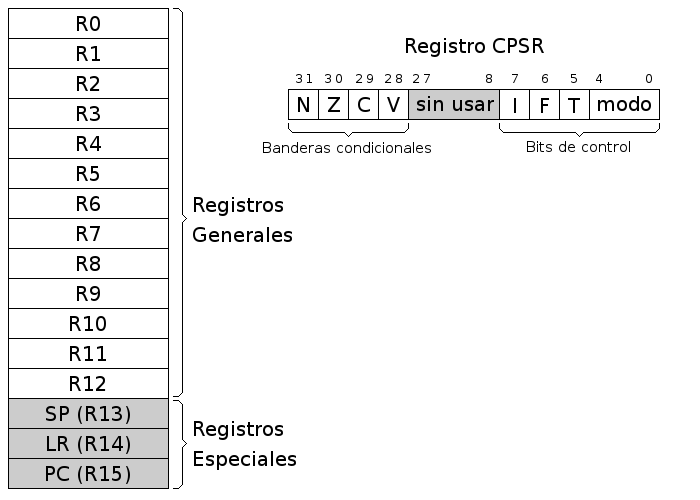
\includegraphics[width=14cm]{graphs/registros.png}
  \caption{Registros de la arquitectura ARM}
  \label{fig:reg_arm}
\end{figure}

\begin{descript}
  \item[Registros Generales.]
    Su función es el almacenamiento temporal de datos. Son los 13 registros
    que van R0 hasta R12.
  \item[Registros Especiales.]
    Son los últimos 3 registros principales: R13, R14 y R15. Como son de
    propósito especial, tienen nombres alternativos.

    \begin{itemize}
      \item{\textbf{SP}/R13. Stack Pointer ó Puntero de Pila. Sirve como puntero para almacenar
        variables locales y registros en llamadas a funciones.}
      \item{\textbf{LR}/R14. Link Register ó Registro de Enlace. Almacena la dirección de retorno
        cuando una instrucción BL ó BLX ejecuta una llamada a una rutina.}
      \item{\textbf{PC}/R15. Program Counter ó Contador de Programa. Es un registro que indica
        la posición donde está el procesador en su secuencia de instrucciones. Se
        incrementa de 4 en 4 cada vez que se ejecuta una instrucción, salvo que ésta
        provoque un salto.}
    \end{itemize}

  \item[Registro CPSR.]
        Almacena las banderas condicionales y los bits de control. Los bits de control
        definen la habilitación de interrupciones normales (I),
        interrupciones rápidas (F), modo Thumb \footnote{es un modo simplificado donde las
        instrucciones son de 16 bits en lugar de 32 y se acceden a menos registros (hasta r7),
        con la ventaja de que el código ocupa menos espacio.} (T) y el modo de operación
        de la CPU. Existen hasta 8 modos de operación, pero desde nuestra aplicación
        sólo vamos a trabajar en uno de ellos, el {\it Modo Usuario}. Los demás son modos
        privilegiados usados exclusivamente por el sistema operativo.

        Desde el {\it Modo Usuario} sólo podemos acceder a las banderas condicionales, que
        contienen información sobre el estado de la última operación realizada por la ALU.
        A diferencia de otras arquitecturas en ARMv6 podemos elegir si queremos que una
        instrucción actualice o no las banderas condicionales, poniendo una "s" detrás
        del nemotécnico \footnote{Es la forma de nombrar las instrucciones desde
        ensamblador, normalmente derivadas de una abreviatura del verbo en inglés. Por
        ejemplo la instrucción {\it MOV} viene de "move" (mover) }. Existen 4 banderas
        y son las siguientes:

    \begin{itemize}
      \item{\textbf{N}. Se activa cuando el resultado es negativo.}
      \item{\textbf{Z}. Se activa cuando el resultado es cero o una comparación es cierta.}
      \item{\textbf{C}. Indica acarreo en las operaciones aritméticas.}
      \item{\textbf{V}. Desbordamiento aritmético.}
    \end{itemize}
\end{descript}


\subsubsection{Esquema de almacenamiento}

El procesador es {\it Bi-Endian}, quiere decir que es configurable entre {\it Big Endian}
y {\it Little Endian}. Aunque nuestro sistema operativo nos lo limita a {\it Little Endian}.

Por tanto la regla que sigue es ''el byte menos significativo ocupa la posición más baja''.
Cuando escribimos un dato en una posición de memoria, dependiendo de si es byte, half word
o word,... se ubica en memoria según el esquema de la figura 1.1. La dirección de un dato
es la de su byte menos significativo. La memoria siempre se referencia a nivel de byte, es
decir si decimos la posición N nos estamos refiriendo al byte N-ésimo, aunque se escriba
media palabra, una palabra,...

***cambiar los textos del .pdf por strb r1, [r0]  strh r1, [r0]  str  r1, [r0]  
\begin{figure}[h]
  \centering
    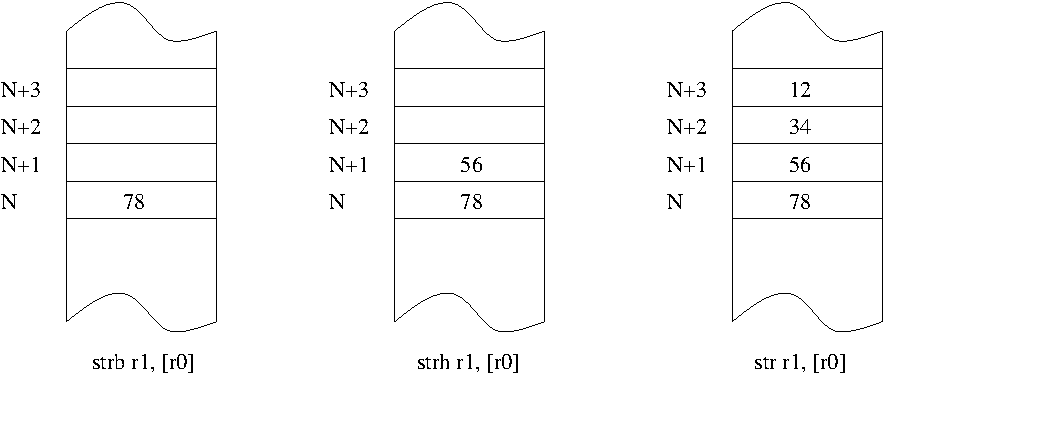
\includegraphics[width=13cm]{graphs/memo.pdf}
  \caption{Ubicación de datos en memoria}
  \label{fig:memo}
\end{figure}

\subsection{El lenguaje ensamblador}

El ensamblador es un lenguaje de bajo nivel que permite un control
directo de la CPU y todos los elementos asociados. Cada línea de un
programa ensamblador consta de una instrucción del procesador y la
posición que ocupan los datos de esa instrucción.

Desarrollar programas en lenguaje ensamblador es un proceso laborioso.
El procedimiento es similar al de cualquier lenguaje compilado.
Un conjunto de instrucciones y/o datos forman un módulo fuente.
Este módulo es la entrada del compilador, que chequea la sintaxis y lo
traduce a código máquina formando un módulo objeto.
Finalmente, un enlazador (montador ó {\it linker}) traduce todas las
referencias relativas a direcciones absolutas.

El ensamblador presenta una serie de ventajas e inconvenientes con
respecto a otros lenguajes de más alto nivel. Al ser un lenguaje de
bajo nivel, presenta como principal característica la flexibilidad y
la posibilidad de acceso directo a nivel de registro. En
contrapartida, programar en ensamblador es laborioso puesto que los
programas contienen un número elevado de líneas y la corrección y
depuración de éstos se hace difícil.

Generalmente, y dado que crear programas un poco extensos es
laborioso, el ensamblador se utiliza como apoyo a otros lenguajes
de alto nivel para 3 tipos de situaciones:
\begin{itemize}
     \item[-] Operaciones que se repitan un número elevado de veces.
     \item[-] Cuando se requiera una gran velocidad de proceso.
     \item[-] Para utilización y aprovechamiento de dispositivos y
     recursos del sistema.
\end{itemize}

\subsection{El entorno}

Los pasos habituales para hacer un programa (en cualquier lenguaje) son 
los siguientes:
lo primero es escribir el programa en el lenguaje fuente
mediante un editor de programas.
El resultado es un fichero en un lenguaje que puede entender el usuario,
pero no la máquina.
Para traducirlo a lenguaje máquina hay que utilizar un programa traductor.
Éste genera un fichero con la traducción de dicho programa, pero todavía
no es un programa ejecutable.
Un fichero ejecutable contiene el programa traducido más una serie de
códigos que debe tener todo programa que vaya a ser ejecutado en una
máquina determinada.
Entre estos códigos comunes se encuentran las librerías del lenguaje.
El encargado de unir el código del programa con el código de estas
librerías es un programa llamado montador ({\it linker}) que genera el
programa ejecutable (ver la figura \ref{fig:entorno})

\begin{figure}[h]
  \centering
    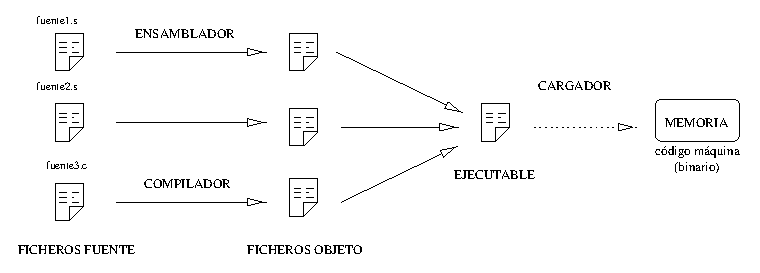
\includegraphics[width=13cm]{graphs/ensamblado.eps}
  \caption{Entorno típico de programación}
  \label{fig:entorno}
\end{figure}

Durante el proceso de creación de un programa se suelen producir errores.
Hay dos tipos de errores: los sintácticos o detectables en tiempo de
traducción y los errores semánticos o detectables en tiempo de ejecución.
Los errores sintácticos son, por ejemplo, escribir mal una instrucción o
hacer una operación entre dos tipos de datos incompatibles.
Estos errores son detectados por el traductor y se deben solucionar para
poder generar un ejecutable.

Una vez que se tiene un programa sintácticamente correcto lo podemos
ejecutar, pero ésto no implica que el programa sea correcto. Todas las
instrucciones pueden ser correctas, pero se puede haber olvidado poner la
condición de salida de un bucle (y que no termine nunca) o que
sencillamente el programa no haga lo que queremos.

Estos errores sólo se pueden detectar en tiempo de ejecución.
Para poder eliminarlos se utiliza un depurador de programas ({\it debugger}).
El depurador nos permite ejecutar el programa instrucción a instrucción y
ver todos los valores que se van a calcular, de manera que podemos encontrar
los errores.

En el laboratorio utilizaremos el editor {\bf nano} para crear
y editar los módulos fuente de nuestros programas. El traductor
(que en el caso de traducir de un lenguaje ensamblador a lenguaje máquina
recibe el nombre de ensamblador), el {\it linker} y el {\it debugger} son
respectivamente GNU Assembler ({\bf AS}), GNU Compiler Collection ({\bf GCC})
y GNU Debbuger ({\bf GDB}). Todas estas herramientas forman parte de la
GNU toolchain que viene instalada por defecto en la mayoría de las distribuciones
basadas en Linux, en concreto Raspbian. Para obtener más información sobre estos
comandos se puede recurrir a la ayuda del sistema con <man as>, <man gcc> y
<man gdb>. Se aconseja que a lo largo de de esta
primera sesión práctica os vayais familiarizando con ambos entornos,
aunque no se os indique explícitamente.

\subsection{Aspecto de un programa en ensamblador}

En el listado \ref{lst:codigoPract1} se muestra el código de la primera
práctica que probaremos. En el código hay una serie de elementos que
aparecerán en todos los programas y que estudiaremos a continuación.

\begin{lstlisting}[caption={Código del programa intro1.s},label={lst:codigoPract1},numbers=left,escapeinside={@}{@}]
.data

var1:   .word   3
var2:   .word   4
var3:   .word   0x1234

.text
.global main
 
main:   ldr     r1, puntero_var1    /* r1 <- &var1    */
        ldr     r1, [r1]            /* r1 <- *r1      */
        ldr     r2, puntero_var2    /* r2 <- &var2    */
        ldr     r2, [r2]            /* r2 <- *r2      */
        ldr     r3, puntero_var3    /* r3 <- &var3    */
        add     r0, r1, r2          /* r0 <- r1 + r2  */
        str     r0, [r3]            /* *r3 <- r0      */
        bx      lr

puntero_var1:   .word   var1
puntero_var2:   .word   var2
puntero_var3:   .word   var3
\end{lstlisting}

La principal característica de un módulo fuente en ensamblador es
que existe una clara separación entre las instrucciones y los
datos. La {\it estructura más general de un módulo fuente} es:

\begin{description}
     \item[* Sección de datos.] Viene identificada por la directiva {\it .data}.
En esta zona se definen todas las variables que utiliza el programa
con el objeto de reservar memoria para contener los valores asignados. Hay que
tener especial cuidado para que los datos estén alineados en palabras de 4 bytes,
sobre todo después de las cadenas. Alinear significa rellenar con ceros el final
de un dato para que el siguiente dato comience en una dirección múltiplo de 4 (con
los dos bits menos significativos a cero). Los datos son modificables.

     \item[* Sección de código.] Se indica con la directiva {\it .text}, y sólo
puede contener código o datos no modificables. Como todas las instrucciones son
de 32 bits no hay que tener especial cuidado en que estén alineadas. Si tratamos
de escribir en esta zona el ensamblador nos mostrará un mensaje de error.
\end{description}

De estas tres secciones la único que obligatoriamente debe existir es
el la sección .text (o sección de código). En el ejemplo \ref{fig:codigoPract1}
comprobamos que están las dos.

Un módulo fuente, como el del ejemplo, está formado por instrucciones,
datos, símbolos y directivas. 
Las instrucciones son representaciones nemotécnicas del juego
de instrucciones del procesador. Un dato es una entidad que aporta un valor
numérico, que puede expresarse en distintas bases o incluso a través de una cadena.
Los símbolos son representaciones abstractas que el ensamblador maneja en tiempo
de ensamblado pero que en el código binario resultante tendrá un valor numérico
concreto. Hay tres tipos de símbolos: las etiquetas, las macros y las constantes simbólicas.
Por último tenemos las directivas, que sirven para indicarle ciertas cosas al
ensamblador, como delimitar secciones, insertar datos, crear macros, constantes
simbólicas, etc... Las instrucciones se aplican en tiempo de ejecución
mientras que las directivas se aplican en tiempo de ensamblado.

\subsubsection{Datos}

Los datos se pueden representar de distintas maneras. Para representar números tenemos
4 bases. La más habitual es en su forma decimal, la cual no lleva ningún delimitador
especial. Luego tenemos otra muy útil que es la representación hexadecimal, que
indicaremos con el prefijo {\it 0x}. Otra interesante es la binaria, que emplea el
prefijo {\it 0b} antes del número en binario. La cuarta y última base es la
octal, que usaremos en raras ocasiones y se especifica con el prefijo {\it 0}. Sí, un
cero a la izquierda de cualquier valor convierte en octal dicho número. Por ejemplo
015 equivale a 13 en decimal. Todas estas bases pueden ir con un signo menos delante,
codificando el valor negativo en complemento a dos. Para representar carácteres y cadenas
emplearemos las comillas simples y las comillas dobles respectivamente.

\subsubsection{Símbolos}

Como las etiquetas se pueden ubicar en tanto en la sección de datos como en la de código,
la versatilidad que nos dan las mismas es enorme. En la zona de datos pueden representar
variables, constantes y cadenas. En la zona de código etiquetas de salto, funciones y
punteros a zona de datos.

Las macros y las constantes simbólicas son símbolos cuyo ámbito pertenece al preprocesador,
a diferencia de las etiquetas que pertenecen al del ensamblador. Se especifican con las
directivas .equ y .macro respectivamente y permiten que el código sea más legible y menos
repetitivo.

\subsubsection{Instrucciones}

Las instrucciones del {\it AS} responden al formato general:


\begin{lstlisting}
Etiqueta:  Nemotécnico  Operando/s  /* Comentario */
\end{lstlisting}

De estos campos, sólo el nemónico (nombre de la instrucción) es obligatorio. En
la sintaxis del {\it AS} cada instrucción ocupa una línea terminando preferiblemente
con el ASCII 10 (LF), aunque son aceptadas las 4 combinaciones: CR, LF, CR LF y LF CR.
Los campos se separan entre sí por al menos un carácter espacio (ASCII 32) o un tabulador
y no existe distinción entre mayúsculas y minúsculas.

\begin{lstlisting}
main:   ldr     r1, puntero_var1    /* r1 <- &var1    */
\end{lstlisting}

El Campo {\it etiqueta}, si aparece, debe estar formado por una
cadena alfanumérica. La cadena no debe comenzar con un dígito y no se puede
utilizar como cadena alguna palabra reservada del {\it AS} ni nombre
de registro del microprocesador. En el ejemplo, la etiqueta es
{\tt 'main:'}.

El campo \textit{Nemotécnico} ({\tt ldr} en el ejemplo) es una forma
abreviada de nombrar la instrucción del procesador.
Está formado por caracteres alfabéticos (entre 1 y 11 caracteres).

El campo \textit{Operando/s} indica dónde se encuentran los datos.
Puede haber 0, 1 ó más operandos en una instrucción. Si hay más de uno
normalmente al primero se le denomina destino (salvo excepciones como {\tt str})
y a los demás fuentes, y deben ir separados por una coma.
Los operandos pueden ser registros, etiquetas, valores inmediatos o incluso
elementos más complejos como desplazadores/rotadores o indicadores de
pre/post-incrementos. En cualquiera de los casos el tamaño debe ser una
palabra (32 bits), salvo contadas excepciones como {\tt ldr} y {\tt str}
donde puede ser media palabra (16 bits) o un byte (8 bits).
En el ejemplo {\tt r1} es el operando destino, de tipo registro,
y {\tt puntero\_var1} es el operando fuente, una etiqueta, ambos
de tamaño palabra (32 bits).

El campo \textit{Comentario} es opcional ({\tt r1 <- \&var1}, en el ejemplo)
y debe comenzar con la secuencia {\tt /*} y acabar con {\tt */} al igual
que los comentarios multilínea en C. No es obligatorio que estén a la
derecha de las instrucciones, aunque es lo habitual. También es común
verlos al comienzo de una función (ocupando varias líneas) para explicar
los parámetros y funcionalidad de la misma.

Cada instrucción del {\it AS} se refiere a una operación que puede
realizar el microprocesador. También hay pseudoinstrucciones que son
tratadas por el preprocesador como si fueran macros y codifican otras
instrucciones, como {\tt lsl rn, \#x} que codifica {\tt mov rn, rn, lsl \#x},
o bien {\tt push/pop} que se traducen instrucciones {\tt stm/ldm} más complejas
y difíciles de recordar para el programador. Podemos agrupar el conjunto de
instrucciones del {\it AS}, según el tipo de función que realice el
microprocesador, en las siguientes categorías:

\begin{itemize}

       \item \textit{Instrucciones de transferencia de datos}
Mueven información entre registros y posiciones de memoria. En la
arquitectura ARMv6 no existen puertos ya que la E/S está mapeada
en memoria. Pertenecen a este grupo las siguientes instrucciones:
\textbf{mov, ldr, str, ldm, stm, push, pop}.

       \item \textit{Instrucciones aritméticas.}  Realizan operaciones
aritméticas sobre números binarios o BCD.  Son instrucciones de este
grupo \textbf{add, cmp, adc, sbc, mul}.

     \item \textit{Instrucciones de manejo de bits.}  Realizan
operaciones de desplazamiento, rotación y lógicas sobre registros o
posiciones de memoria. Están en este grupo las instrucciones:\textbf{
and, tst, eor, orr, lsl, lsr, asr, ror, rrx}.

     \item \textit{Instrucciones de transferencia de control.}  Se
utilizan para controlar el flujo de ejecución de las instrucciones
del programa. Tales como \textbf{b, bl, bx, blx} y sus variantes
condicionales.

\end{itemize}

En esta sesión práctica se explorarán algunas de estas instrucciones.
Para buscar información sobre cualquiera de ellas durante las prácticas,
recuerda que puedes utilizar el datasheet del ARM1176JZF-S.

\subsubsection{Directivas}

Las directivas son expresiones que aparecen en el módulo fuente e
indican al compilador que realice determinadas tareas en el proceso
de compilación. Son fácilmente distinguibles de las instrucciones
porque siempre comienzan con un punto. El uso de directivas es
aplicable sólo al entorno del compilador, por tanto varían de un
compilador a otro y para diferentes versiones de un mismo compilador.
Las directivas más frecuentes en el {\it AS} son:

\begin{itemize}
        \item \textit{Directivas de asignación:} Se utilizan para dar
valores a las constantes o reservar posiciones de memoria para las
variables (con un posible valor inicial).  \textbf{.byte, .hword, .word,
.ascii, .asciz, .zero y .space}
son directivas que indican al compilador que reserve memoria para
las variables del tipo indicado. Por ejemplo,

\begin{lstlisting}
a1:   .byte  1       /* tipo byte, inicializada a 1 */
var2: .byte  'A'     /* tipo byte, al caracter 'A'  */
var3: .hword 25000   /* tipo hword (16 bits) a 25000*/
var4: .word 0x12345678 /* tipo word de 32 bits      */
b1:   .ascii "hola"  /* define cadena normal        */
b2:   .asciz "ciao"  /* define cadena acabada en NUL*/
dat1: .zero  300     /* 300 bytes de valor cero     */
dat2: .space 200, 4  /* 200 bytes de valor 4        */
\end{lstlisting}

La directiva \textbf{.equ} (ó \textbf{.set}) es utilizada para asignar un
valor a una constante simbólica.

\begin{lstlisting}
.equ N, -3     /* en adelante N se sustituye por -3 */
\end{lstlisting}

\item \textit{Directivas de control:}
        \textbf{.text y .data} sirven para delimitar las distintas secciones
        de nuestro módulo.
        \textbf{.align {alineamiento}} es para alinear el siguiente dato,
        rellenando con ceros, de tal forma que comience en una dirección
        múltiplos del número que especifiquemos en {\it alineamiento},
        normalmente potencia de 2. Si no especificamos {\it alineamiento}
        por defecto toma el valor de 4 (alineamiento a palabra).

\begin{lstlisting}
a1: .byte 25   /* definimos un byte con el valor 25 */
    .align     /* directiva que rellena con 3 bytes */
a2: .word 4    /* variable alineada a tamaño palabra*/
\end{lstlisting}

        \textbf{.include} para incluir un archivo fuente dentro del actual.
        \textbf{.global} hace visible al enlazador el símbolo que hemos
        definido con la etiqueta del mismo nombre.

     \item \textit{Directivas de operando:} Se aplican a los datos en
        tiempo de compilación. En general, incluyen las operaciones lógicas
        {\tt \&}, {\tt |}, {\tt \~{}}, aritméticas {\tt +}, {\tt -},
        {\tt *}, {\tt /}, {\tt \%} y de desplazamiento
        {\tt $<$}, {\tt $>$}, {\tt $<<$}, {\tt $>>$}.

\begin{lstlisting}
.equ pies, 9     /* definimos a 9 la constante pies */
.equ yardas, pies/3     /* calculamos las yardas= 3 */
.equ pulgadas, pies*12  /* calculamos pulgadas= 108 */
\end{lstlisting}

     \item \textit{Directivas de Macros:} Una {\it .macro} es un
conjunto de sentencias en ensamblador (directivas e instrucciones) que
pueden aparecer varias veces repetidas en un programa con algunas
modificaciones (opcionales). Por ejemplo, supongamos que a lo largo de
un programa realizamos varias veces la operación $n^{2}+1$ donde n y el
resultado son registros. Para acortar el código a escribir
podríamos usar una macro como la siguiente:

\begin{lstlisting}
    .macro CuadM1 input, aux, output
        mul     aux, input, input
        add     output, aux, #1
    .endm    
\end{lstlisting}

Esta macro se llama {\it CuadM1} y tiene tres parámetros (input, aux y output).
Cada vez que la usemos en el programa haremos:

\begin{lstlisting}
        CuadM1  r1, r8, r0
\end{lstlisting}

\noindent y el ensamblador {\it expande} la macro, es decir, en lugar de
la llamada coloca:

\begin{lstlisting}
        mul     r8, r1, r1
        add     r0, r8, #1
\end{lstlisting}

No hay que confundir las macros con los procedimientos. Por un lado,
el código de un procedimiento es único, todas las llamadas usan el
mismo, mientras que el de una macro aparece (se expande) cada vez que
se referencia, por lo que ocuparán más memoria. Las macros serán
más rápidas en su ejecución, pues es secuencial, frente a la de
los procedimientos, ya que implican un salto cuando aparece la llamada
y un retorno cuando se termina. La decisión de usar una macro o un
procedimiento dependerá de cada situación en concreto, aunque las
macros son muy flexibles (ofrecen muchísimas más posibilidades de las
comentadas aquí). Esta posibilidad será explotada en sesiones más avanzadas.

\end{itemize}

\subsection{Ensamblar y {\it linkar} un programa}

La traducción o ensamblado de un módulo fuente ({\bf nombreprograma.s})
se realiza con el programa Gnu Assembler, con el siguiente comando:

\hspace{2.5cm}{\bf as -o nombreprograma.o nombreprograma.s}

NOTA: tanto el comando {\it as} como el nombre del programa son sensibles
a las mayúsculas. Por tanto el comando debe ir en minúsculas y el nombre
como queramos, pero recomendamos minúsculas también.
Las opción {\bf -o nombreprograma.o} puede ir después de {\bf nombreprograma.s}.

El {\it as} genera un fichero nombreprograma.o.

Para montar ({\it linkar}) hay que hacer:

\hspace{2.5cm}{\bf gcc -o nombreprograma nombreprograma.o}

NOTA: Nuevamente, tanto {\it gcc} como el nombre del programa deben estar
en minúsculas. Este comando es muy parecido al anterior, podemos poner si
queremos {\bf -o nombreprograma} detrás de {\bf nombreprograma.o}. La única
diferencia es que el archivo no tiene extensión, que por otro lado es una
práctica muy recomendable para ejecutables en Linux.

Una vez hecho ésto, ya tenemos un fichero ejecutable (nombreprograma) que
podemos ejecutar o depurar con el {\it gdb}.


\chapterend{}

%%%%%%%%%%%%%%%%%%%%%%%%%%%%%%%%%%%%%%%%%%%%%%%%%%%%%%%%%%%%%%
\end{document}